To train the sparse autoencoder described in Section \ref{section:dictionary_learning}, we use data from the Pile \citep{gao2020pile}, a large, public webtext corpus. We run the model that we want to interpret over this text while caching and saving the activations at a particular layer. These activations then form a dataset, which we use to train the autoencoders. The autoencoders are trained with the Adam optimiser with a learning rate of 1e-3 and are trained on 5-50M activation vectors for 1-3 epochs, with larger dictionaries taking longer to converge. A single training run using this quantity of data completes in under an hour on a single A40 GPU.

When varying the hyperparameter $\alpha$ which controls the importance of the sparsity loss term, we consistently find a smooth tradeoff between the sparsity and accuracy of our autoencoder, as shown in Figure \ref{fig:smooth_trade}. The lack of a `bump' or `knee' in these plots provides some evidence that there is not a single correct way to decompose activation spaces into a sparse basis, though to confirm this would require many additional experiments. Figure \ref{fig:trade_over_time} shows the convergence behaviour of a set of models with varying $\alpha$ over multiple epochs.
 
\begin{figure}[hb]
    \centering
    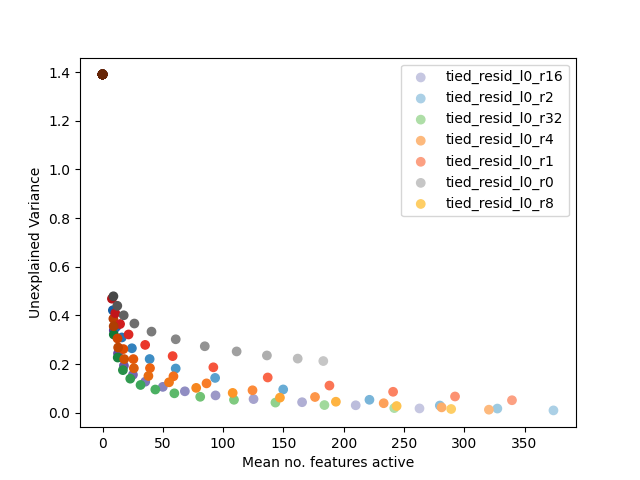
\includegraphics[width=.9\textwidth]
    {images/sizes_place.png}
    \caption{The tradeoff between the average number of features active and the proportion of variance that is unexplained for the MLP at layer 0.}
    \label{fig:smooth_trade}
\end{figure}


\begin{figure}
    \centering
    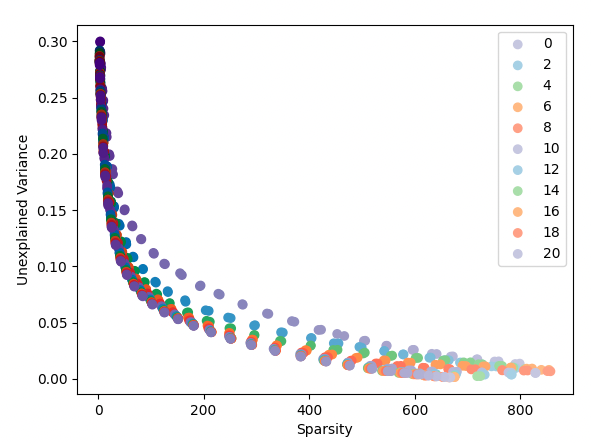
\includegraphics[width=0.9\textwidth]{images/overtime_place.png}
    \caption{The tradeoff between sparsity and unexplained variance in our reconstruction. Each series of points is a sweep of the $\alpha$ hyperparameter, trained for the number of epochs given in the legend.}
    \label{fig:trade_over_time}
    % \label{fig:overtime_place}
\end{figure}
